\documentclass[../NFTComp_IEEE.tex]{subfiles}
\graphicspath{{\subfix{../Images}}}

\begin{document}
\section{Development of a NFT Smart Contract in Cadence}
\label{sec:cadence_development}
The present section assumes a minimal knowledge from the reader about general blockchain technology and NFT development in Solidity. As such, we opt to omit the implementation details from this blockchain and focus the text on the unfamiliar Cadence version. Fig. \ref{fig:cadence_nft_contract} presents a schematic representation of the contract developed. It displays required standard dependencies and the functions and fields required by this inheritance.

\begin{figure}[h!]
    \centering
    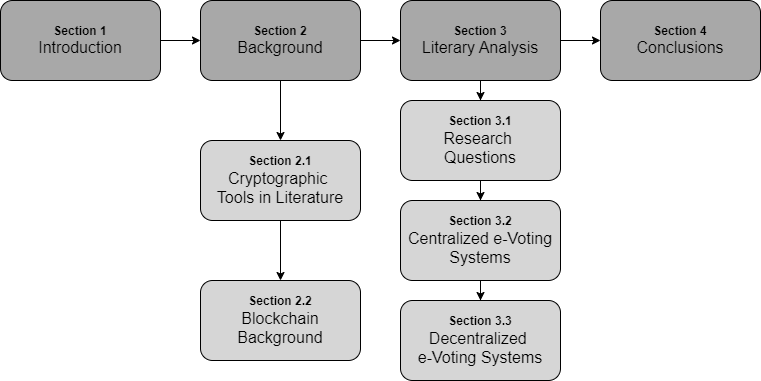
\includegraphics[width=\columnwidth]{Images/almei1.png}
    \caption{Structural organisation of an NFT smart contract in Cadence}
    \label{fig:cadence_nft_contract}
\end{figure}

\subsection{Imported Standards}
The simplest standardised version of a Cadence NFT smart contract requires the import of two standards, namely, the \textit{NonFungibleToken} and \textit{MetadataViews} interfaces. We omitted references to the \textit{MetadataViews} because this import is an imposition from the \textit{NonFungibleToken} import. Flow is particularly suited for applications with high NFT throughput, such as digital collectibles. The \textit{MetadataViews} standard is used mostly to support metadata operations, which are used extensively in Flow to compose digital collectible objects similar to trading cards. This functional aspect falls outside the bounds of this study; therefore, we implemented the required functions from this standard as stubs. Fig. \ref{fig:cadence_nft_contract} uses a colour scheme to indicate which standard required the function, resource, and event indicated in the contract structure.

\subsubsection{Resources}
The \textit{NonFungibleToken} standard requires the implementation of NFTs and a collection resource as minimal requirements. But Fig. \ref{fig:cadence_nft_contract} shows a third resource in the contract, namely a \textit{NFTMinter} resource used to abstract, simplify, and secure the minting of new NFTs. New resources can only be created with a contract function due to Cadence restricting the "\textbf{create}" keyword to the context of the contract. Transactions are not able to invoke this internal action by themselves. A secure and simple approach to resource creation is to define the create function inside of another resource and create and save it to the owner's account storage in the contract constructor. Only the owner can create new NFTs, since he/she is the only one with access to the account storage. This effectively decouples the creation of NFTs from the contract itself.

\subsubsection{Functions}
The \textit{NonFungibleToken} standard requires the implementation of a \textit{createEmptyCollection} function to obtain a collection resource, but it also requires similar implementations in the NFT and even in the collection resource itself. Standard NFT contracts in Flow provide multiple access points to create new collections. The \textit{createEmptyCollection} function at the contract level requires a type as input because it is not possible to infer the storage type at that level. Versions at the resource level infer the storage type from the resource housing it.

\subsubsection{Events}
A contract that imports the \textit{NonFungibleToken} inherits the \textit{Withdrawn} and \textit{Deposited} events by default. In Cadence, like in Solidity, importing standards implements and emits imported events automatically. Events imported from standards do not require explicit implementation in contracts, unlike functions and resources. Whenever an ExampleNFT moves in or out of storage, the events in Fig. \ref{fig:cadence_nft_contract} emit automatically.
\end{document}